\documentclass{beamer}

\usepackage[utf8]{inputenc}
\usepackage[T1]{fontenc}
\usepackage[french]{babel}
\usepackage{fontspec}
\usepackage{csquotes}

% colors
\definecolor{palepink}{rgb}{0.98, 0.85, 0.87}
\definecolor{plum}{rgb}{0.44, 0.11, 0.11}
\definecolor{lilac}{rgb}{0.8, 0.8, 1.0}
\definecolor{peachpuff}{rgb}{1.0, 0.85, 0.73}
\definecolor{lightpink}{rgb}{1.0, 0.71, 0.76}
\definecolor{pearl}{rgb}{0.94, 0.92, 0.84}
\definecolor{lightmauve}{rgb}{0.86, 0.82, 1.0}
\definecolor{cherryblossompink}{rgb}{1.0, 0.72, 0.77} 	
\definecolor{nadeshikopink}{rgb}{0.96, 0.68, 0.78}
\definecolor{pastelviolet}{rgb}{0.8, 0.6, 0.79}
\definecolor{moccasin}{rgb}{0.98, 0.92, 0.84}
\definecolor{persimmon}{rgb}{0.93, 0.35, 0.0}
\definecolor{electricpurple}{rgb}{0.75, 0.0, 1.0}
\definecolor{wildstrawberry}{rgb}{1.0, 0.26, 0.64}
\definecolor{outrageousorange}{rgb}{1.0, 0.43, 0.29}
\definecolor{darkterracotta}{rgb}{0.8, 0.31, 0.36}

% captions
\usepackage{subcaption}
\usepackage{caption}
\DeclareCaptionFormat{custom}{%
	\scriptsize{#1#2#3}
}
\captionsetup{format=custom,width=0.8\textwidth}

% tikz
\usepackage{tikz}
\usetikzlibrary{shapes.geometric}
\tikzstyle{base} = [%
	draw,%
	rectangle,%
	rounded corners=3pt,%
	minimum height=1cm,%
	fill=lilac,%
	draw=plum,%
	text centered,%
	text width=4cm%
]
\tikzstyle{db} = [%
	cylinder,%
	shape border rotate=90,%
	aspect=0.25,%
	fill=pastelviolet,%
	draw=plum,%
	text centered,%
	text width=4cm%
]
\tikzstyle{transf} = [%
	trapezium,%
	trapezium left angle=70,%
	trapezium right angle=110,%
	minimum height=1cm,%
	fill=lightpink,%
	draw=plum,%
	text centered,%
	text width=3cm%
]
\tikzstyle{choice} = [%
	diamond,%
	minimum width=2cm,%
	aspect=2,%
	fill=peachpuff,%
	draw=plum,%
	text centered,%
	text width=4cm%
]
\tikzstyle{expl} = [%
	rectangle,%
	draw=plum,%
	fill=moccasin,%
	text centered,%
	text width=4cm%
]
\tikzstyle{outline} = [%
	rectangle,%
	rounded corners,%
	draw=plum,%
	text width=4cm,%
	ultra thick
]
\tikzstyle{outline-no-width} = [%
	rectangle,%
	rounded corners,%
	draw=plum,%
	ultra thick
]
\tikzstyle{blank} = [%
	rectangle,%
	draw=white,%
	draw opacity=0%
]
\tikzstyle{arrow} = [%
	thick,%
	->,%
	>=stealth,%
	color=plum%	
]
\tikzstyle{doublearrow} = [%
	thick,%
	<->,%
	>=stealth,%
	color=plum,%
]
\tikzstyle{line} = [%
	thick,%
	color=plum%	
]
\tikzstyle{dotted} = [%
	thick,%
	->,%
	>=stealth,%
	color=plum,%
	dash pattern=on 3pt off 4pt on \the\pgflinewidth off 4pt%
]
\pgfdeclarelayer{bg}    % declare background layer
\pgfsetlayers{bg,main}  % set the order of the layers (main is the standard layer)


\usepackage[newfloat]{minted}
\SetupFloatingEnvironment{listing}{name=D\scriptsize{ONNÉES BRUTES}}
\usemintedstyle{borland}
\setminted{linenos, breaklines, tabsize=4, bgcolor=lightmauve,fontsize=\tiny}

\definecolor{lightmauve}{rgb}{0.86, 0.82, 1.0}

\title{Modélisation, enrichissement sémantique et diffusion d'un corpus textuel semi-structuré: le cas des catalogues de vente de manuscrits.}
\date{25 septembre 2022}
\author[Paul H. Kervegan]{Paul, Hector Kervegan}

\usetheme{hector}

\usepackage{hyperref}
\hypersetup{
	colorlinks=true,
	linkcolor=wildstrawberry,
	filecolor=wildstrawberry,
	citecolor=wildstrawberry,      
	urlcolor=wildstrawberry,
	pdfauthor={Paul, Hector KERVEGAN}, 
	pdftitle={Modélisation, enrichissement sémantique et diffusion d'un corpus textuel semi-structuré: le cas des catalogues de vente de manuscrits (soutenance)}, 
	pdfsubject={Traitement de données textuelles},
	pdfkeywords={catalogues de vente}{mss}{katabase}{ocr}{web sémantique}{linked open data}{web de données}{traitement automatisé du language}{détection de motifs}{api}{fair}{rest}
}

\begin{document}
	
% present the outline at search section change
\AtBeginSection{
	\begin{frame}{Plan}
		\tableofcontents[currentsection]
	\end{frame}
}

\begin{frame}
	\titlepage
\end{frame}

\begin{frame}
	\frametitle{Introduction}
	\framesubtitle{Problématique}
	
	En quoi la nature semi-structurée du corpus permet d'en automatiser le traitement? Comment produire des informations normalisées et exploitables à partir d'un corpus textuel semi-structuré? Comment rendre la recherche en humanités numériques réutilisable et encourager le partage de données entre projets de recherche?
\end{frame}

\begin{frame}
	\frametitle{Introduction}
	\framesubtitle{Plan}
	\tableofcontents
\end{frame}


\section{La structure du texte comme méthode d'approche}
\subsection{Structure du document et modélisation}
\begin{frame}
	\frametitle{La structure du texte comme méthode d'approche}
	\framesubtitle{Structure du document et modélisation}
	
	Étudier la structure du texte permet de faire le lien entre un document physique et son édition numérique.
	
	
	\begin{figure}[h]
		\centering
		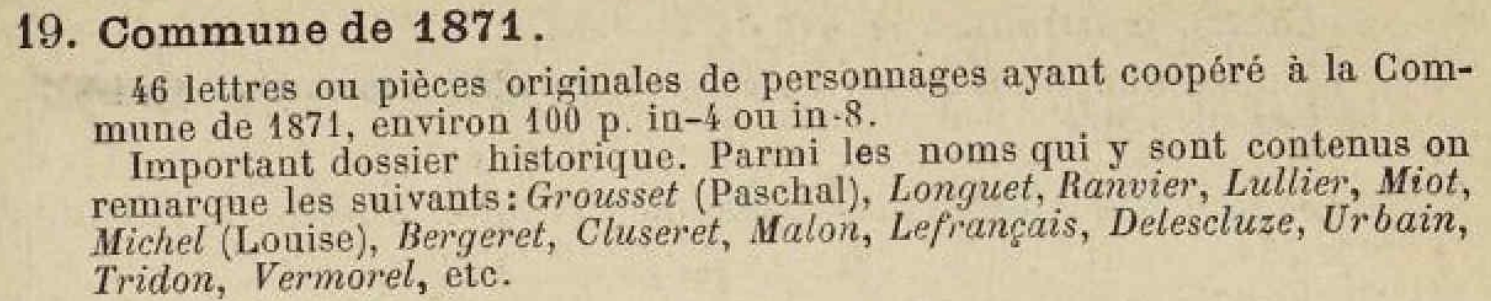
\includegraphics[width=\textwidth]{includes/tei_item.png}
		\caption{Un manuscrit vendu aux enchères}
	\end{figure}
\end{frame}

\begin{frame}
	\frametitle{La structure du texte comme méthode d'approche}
	\framesubtitle{Structure du document et modélisation}
	
	\begin{listing}[h]
		\centering
		\inputminted{xml}{includes/tei_item.xml}
		\caption{L'encodage du même manuscrit en \texttt{TEI}}
	\end{listing}
\end{frame}

\subsection{La spécificité d'un corpus \enquote{semi-structuré}}
\begin{frame}
	\frametitle{La structure du texte comme méthode d'approche}
	\framesubtitle{La spécificité d'un corpus \enquote{semi-structuré}}
	
	\enquote{Semi-structuré}, qu'est-ce que ça veut dire?
	\begin{figure}[h]
		\centering
		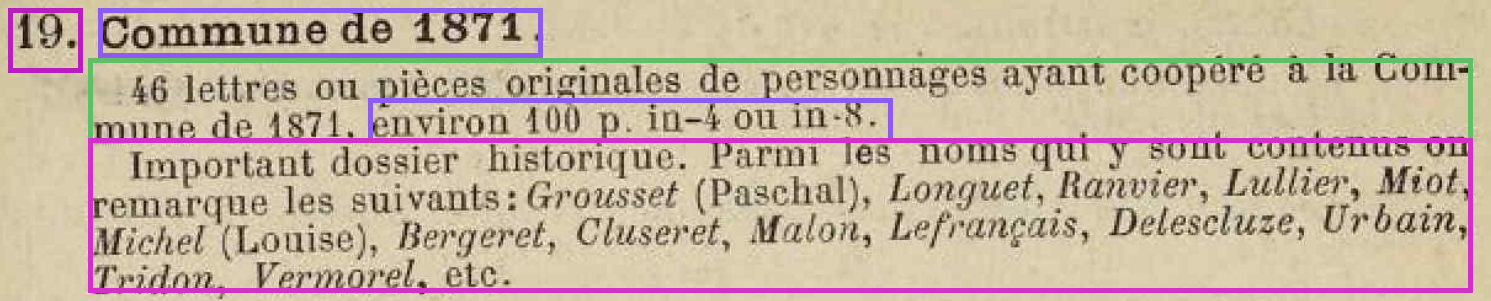
\includegraphics[width=\textwidth]{includes/tei_item_zone.png}
		\caption{Les différents éléments dans la description du manuscrit}
	\end{figure}
\end{frame}

\begin{frame}
	\frametitle{La structure du texte comme méthode d'approche}
	\framesubtitle{La spécificité d'un corpus \enquote{semi-structuré}}
	
	L'édition critique, un autre type de structure formelle pour le texte
	\begin{figure}[h]
		\centering
		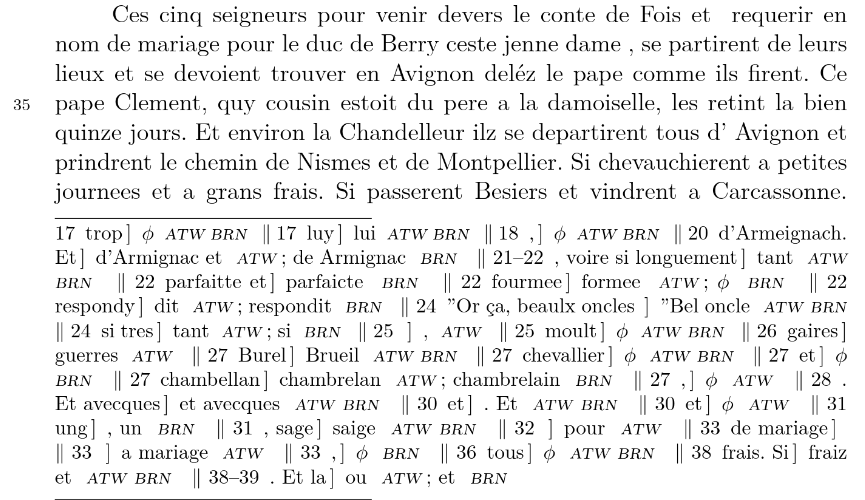
\includegraphics[height=0.4\textheight]{includes/textcrit.png}
		\caption{Extrait d'une édition critique de trois témoins du SHF 3A-306 \enquote{La négogiation du mariage du Duc de Berry} des \textit{Chroniques} de Froissart.}
	\end{figure}
\end{frame}

\section{Sous quels angles aborder cette problématique?}
\subsection{Modéliser un corpus semi-structuré}
\begin{frame}
	\frametitle{Sous quels angles aborder cette problématique?}
	\framesubtitle{Modéliser un corpus semi-structuré}
	
	Modéliser un document revient à identifier sa structure et à l'expliciter à l'aide d'une structure formelle explicite.
	\begin{listing}[h]
		\centering
		\inputminted{xml}{includes/tei_item.xml}
		\caption{L'encodage du même manuscrit en \texttt{TEI}}
	\end{listing}
\end{frame}

\begin{frame}
	\frametitle{Sous quels angles aborder cette problématique?}
	\framesubtitle{Modéliser un corpus semi-structuré}
	
	Les limites de la modélisation
	\begin{figure}[h]
		\centering
		\tikz[transform shape,scale=0.5]{
			\node[name=c, circle,draw=plum,fill=lightmauve,minimum width=5cm, text width=5cm] (c) at (0,0) %
			{\begin{center}\textbf{Différentes significations \\ du texte}\end{center}};
			\foreach \a / \p / \t in {
				north/above/Texte comme idée et comme contenu,
				north east/right/Texte comme œuvre et structure rhétorique,
				south east/right/Texte comme objet linguistique et comme suite de mots,
				south/below/Texte comme ensemble de caractères avec particularités graphiques,
				south west/left/Texte comme document physique individuel,
				north west/left/Texte comme objet visuel et comme signe complexe
			}
			\draw[shift=(c.\a)] plot[mark=*] coordinates{(0,0)} node[\p=0.5cm,text width=4cm] {\t};
		}
		\caption{Les différentes signification d'un texte selon P. Sahle (2016)}
		\label{fig:wheeloftext}
	\end{figure}
\end{frame}

\subsection{Analyser le texte à partir de sa structure: la résolution d'entités nommées}
\begin{frame}
	\frametitle{Sous quels angles aborder cette problématique?}
	\framesubtitle{Analyser le texte à partir de sa structure}
	
	La résolution d'entités nommées à partir de détection de motifs
	\begin{figure}[h!]
		\centering
		\tikz[transform shape,scale=0.68]{
			\node[%
				outline-no-width,%
				draw=nadeshikopink,%
				label={below:nom de famille noble}%
			]%
			at (-10.5,0)%
			{Turenne};
			\node[outline-no-width,draw=white]%
			at (-8.5,0)%
			{(};
			\node[%
				outline-no-width,%
				draw=purple,%
				label={below:prénom}
			]%
			at (-7.25,0)%
			{Henri};
			\node[outline-no-width,draw=white]%
			at (-5.5,0)%
			{de la};
			\node[%
				outline-no-width,%
				draw=red,%
				label={below:nom de famille usuel}]%
			at (-2.5,0)%
			{Tour d'Auvergne};
			\node[%
				outline-no-width,%
				draw=orange,%
				label={below:titre de noblesse}%
			]%
			at (1.3,0)%
			{vicomte};
			\node[outline-no-width,draw=white]%
			at (3,0)%
			{de)};
		}
		\caption{Les différents motifs dans un nom propre}
		\label{code:prepin_teiname_part}
	\end{figure}
\end{frame}

\subsection{Remodeler, re-modéliser le texte pour une API}
\begin{frame}
	\frametitle{Sous quels angles aborder cette problématique?}
	\framesubtitle{Remodeler, re-modéliser le texte pour une API}
	
	Entre texte et données, les catalogues de vente sont des sources utiles pour constituer une API:
	\begin{itemize}
		\item Les descriptions de manuscrits sont quelque part entre texte et donnée
		\item Ils sont composés de plusieurs entités signifiantes en elles-mêmes
		\item Constituer une API permet de créer de nouveaux points d'entrée dans les catalogues
	\end{itemize}
\end{frame}

\section{Le traitement automatique du texte comme chaîne éditoriale continue}
\subsection{L'enrichissement progressif du texte}
\begin{frame}
	\frametitle{Une chaîne éditoriale continue}
	\framesubtitle{L'enrichissement progressif du texte}
	
	Contrairement à une édition papier, une édition numérique est vouée à être continuellement enrichie.
	\begin{listing}[h]
		\centering
		\inputminted{xml}{includes/tei_item_simple.xml}
		\caption{Une description de manuscrit au début de la chaîne de traitement}
	\end{listing}
\end{frame}

\begin{frame}
	\frametitle{Une chaîne éditoriale continue}
	\framesubtitle{L'enrichissement progressif du texte}
	
	\begin{listing}[h]
		\centering
		\inputminted{xml}{includes/tei_item.xml}
		\caption{La même description à la fin de la chaîne de traitement}
	\end{listing}
\end{frame}

\subsection{La résolution d'entités nommées: mettre le texte en réseau}
\begin{frame}
	\frametitle{Une chaîne éditoriale continue}
	\framesubtitle{La résolution d'entités nommées: mettre le texte en réseau}
	
	La résolution d'entités nommées permet de connecter le texte à d'autres données dans une logique d'hypertexte.
\end{frame}

\subsection{Recomposer le texte et créer des documents via une API}
\begin{frame}
	\frametitle{Une chaîne éditoriale continue}
	\framesubtitle{Recomposer le texte et créer des documents via une API}
	
	\begin{listing}[h]
		\centering
		\inputminted{xml}{includes/api.xml}
		\caption{Description d'une requête faite à l'API.}
	\end{listing}
\end{frame}

\begin{frame}
	\frametitle{Conclusion}
	
	Comment la modélisation et l'éditorialisation continue du texte impactent celui-ci?
	\begin{itemize}
		\item L'encodage comme \enquote{métatexte}
		\item L'API et les limites d'une conception traditionnelle du texte
	\end{itemize}
\end{frame}

\end{document}
